\documentclass{beamer}


% \usepackage{CJKnumb}\usepackage{beamerthemesplit}

\mode<article>
{
  \usepackage{beamerbasearticle}
  \usepackage{fullpage}
  \usepackage{hyperref}
}

\usepackage{algorithm}
\usepackage{algorithmic}

%\usepackage{beamerthemesplit} 
%\usepackage{beamerthemeshadow}  
%\usepackage[width=2cm,dark,tab]{beamerthemesidebar}


% Setup appearance:

%\usetheme{Darmstadt}
\usefonttheme[onlylarge]{structurebold}
\setbeamerfont*{frametitle}{size=\normalsize,series=\bfseries}
\setbeamertemplate{navigation symbols}{}

\renewcommand\arraystretch{1.5}

% Standard packages

\usepackage[english]{babel}
%\usepackage[latin1]{inputenc}

\usepackage{epsf}
\usepackage{amsmath,amssymb}
\usepackage{graphicx}
\usepackage{tabularx}

% \usepackage[usenames,dvipsnames]{color}
\definecolor{shadow}{gray}{0.8}
\newcommand{\redc}[1]{{\color{red} #1}}
\newcommand{\bluec}[1]{{\color{blue} #1}}
\newcommand{\shadowc}[1]{{\color{shadow} #1}}
\newcommand{\whitec}[1]{{\color{white} #1}}
\definecolor{myyellow}{HTML}{FFB700}
\newcommand{\yellowc}[1]{{\color{myyellow} #1}}
\newcommand{\greenc}[1]{{\color{green} #1}}
\newcommand{\vect}[1]{\textbf{\textit{#1}}}
\newcommand{\dd}[1]{\textrm{d}}
\newcommand{\corr}{C^{(3)}}

\newcommand{\AT}{{\textrm{{AT}}}}
\newcommand{\EX}{{\textrm{EX}}}
\newcommand{\CG}{{\textrm{CG}}}
\newcommand{\HY}{{\textrm{HY}}}
\newcommand{\thf}{{\textrm{th}}}
\newcommand{\rdf}{{\textrm{rdf}}}

\usepackage{amsfonts}
\newcommand{\tickYes}{\checkmark}
\usepackage{pifont}
\newcommand{\tickNo}{\hspace{1pt}\ding{55}}

% \usetheme{Boadilla}
% \usetheme{Copenhagen}
% \usetheme{Madrid}
\usetheme{Singapore}


\begin{document}
\title[]{
  Grand-Canonical-Like Molecular Dynamics  by Using an
  Adaptive-Resolution Technique
}
%
\author{Han Wang}
\institute[FUB] {
  Institute for Mathematics, Freie Universit\"at Berlin, Germany\\
  % Institut f\"ur Mathematik, Freie Universit\"at Berlin, Germany\\
\vskip 0.4cm
Joint with: Carsten Hartmann, Christof Sch\"utte, Luigi Delle Site (FUB) }
\date[2013]{13 March 2013\\ DPG Spring Meeting, Regensburg}
\frame{\titlepage}

\begin{frame}{AdResS: an overview}
  \redc{AdResS} = \redc{Ad}aptive \redc{Res}olution \redc{S}imulation
  \begin{figure}
    \centering 
    \includegraphics[width=0.6\textwidth]{fig/system.example/example-1.eps}
    % 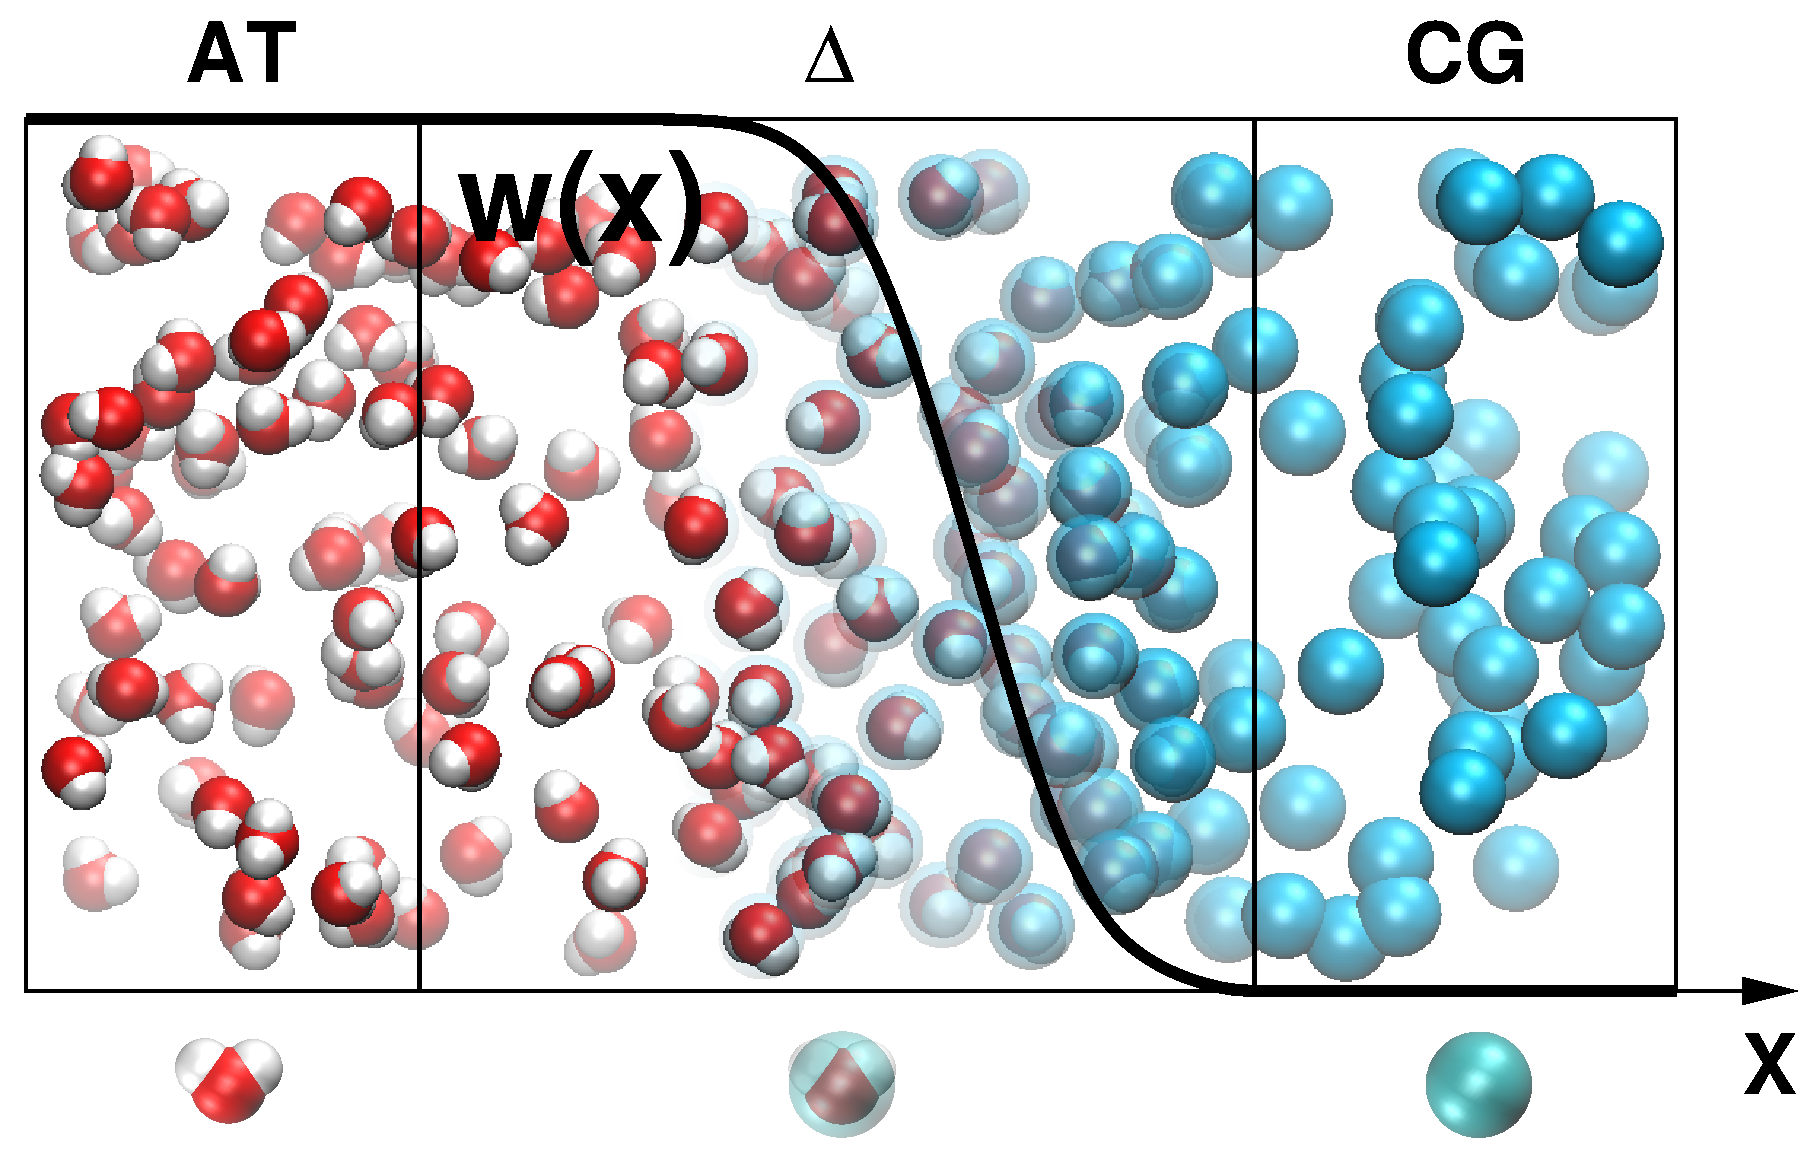
\includegraphics[width=0.8\textwidth]{fig/adapt-wat.eps}
  \end{figure}
  \footnotesize{With courtesy of Luigi Delle Site}
\end{frame}

\begin{frame}{AdResS: an overview}
  \redc{AdResS} = \redc{Ad}aptive \redc{Res}olution \redc{S}imulation
  \begin{figure}
    \centering 
    \includegraphics[width=0.6\textwidth]{fig/system.example/example-2.eps}
    % 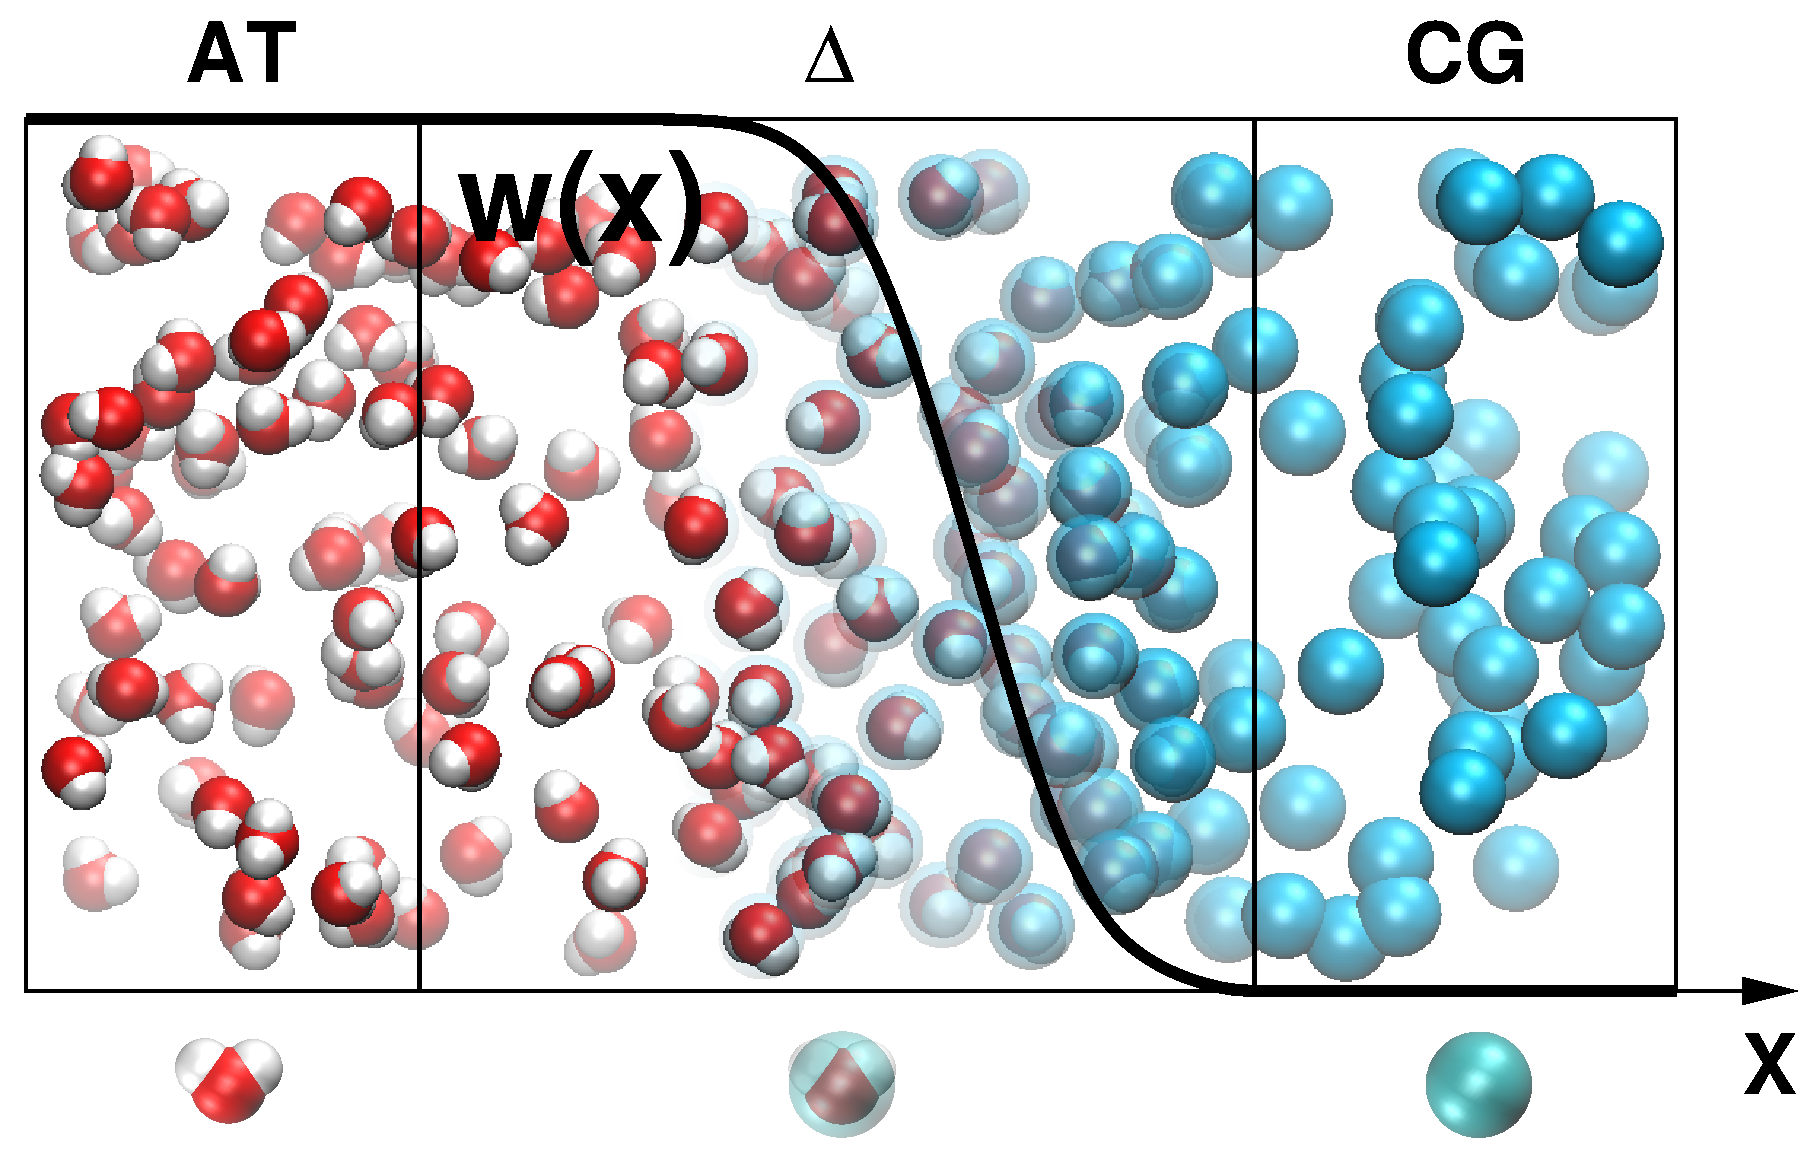
\includegraphics[width=0.8\textwidth]{fig/adapt-wat.eps}
  \end{figure}  
  \footnotesize{With courtesy of Luigi Delle Site}
\end{frame}


\begin{frame}{AdResS: an overview}
  \begin{itemize}
  \item <1-> The weighting function $w(x)$.
  \vskip -.1cm
  \begin{figure}
    \centering 
    \includegraphics[width=0.6\textwidth]{fig/system/system-oldw.eps}
    % 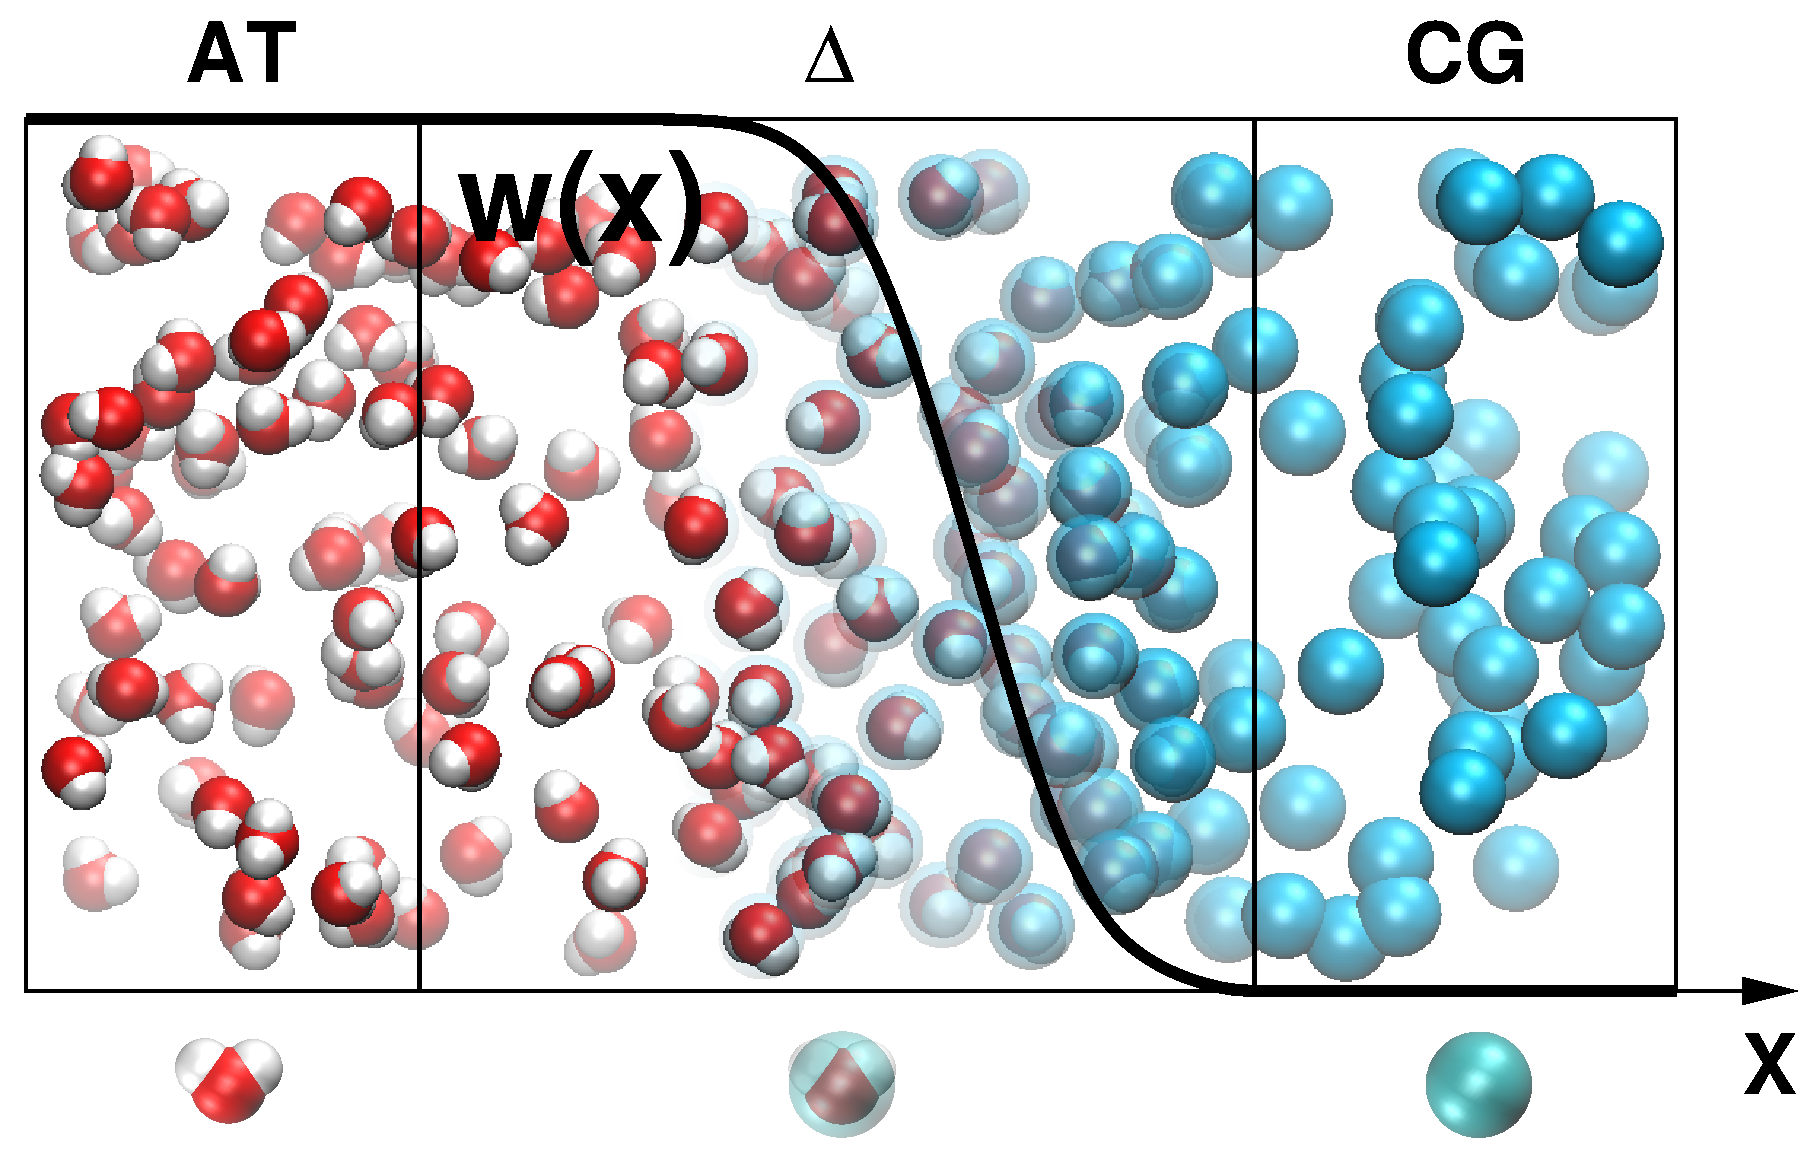
\includegraphics[width=0.8\textwidth]{fig/adapt-wat.eps}
  \end{figure}
  \vskip -.3cm
  \item<2-> Force interpolation scheme:
    \vskip -.6cm
  \begin{align*}
    {\vect F}_{\alpha \beta}&=w_\alpha w_\beta{\vect F}_{\alpha\beta}^{\AT}+[1-w_\alpha w_\beta]{\vect F}^{\CG}_{\alpha\beta} \whitec{\:+\: w_\alpha w_\beta (1-w_\alpha w_\beta)\vect F_{\alpha\beta}^{\rdf}}\\
    {\vect F}_{\alpha }& = \sum_{\beta}{\vect F}_{\alpha \beta} \whitec{\:+\:\vect F^\thf_{\alpha}}
  \end{align*}

  \end{itemize}
  % \footnote{M. Praprotnik, L. Delle Site, K. Kremer, JCP \textbf{123}, 224106 (2005)}
\end{frame}


\begin{frame}{AdResS: an overview}
  \begin{itemize}
  \item <1-> The weighting function $w(x)$.
  \vskip -.1cm
  \begin{figure}
    \centering 
    \includegraphics[width=0.6\textwidth]{fig/system/system-oldw.eps}
    % 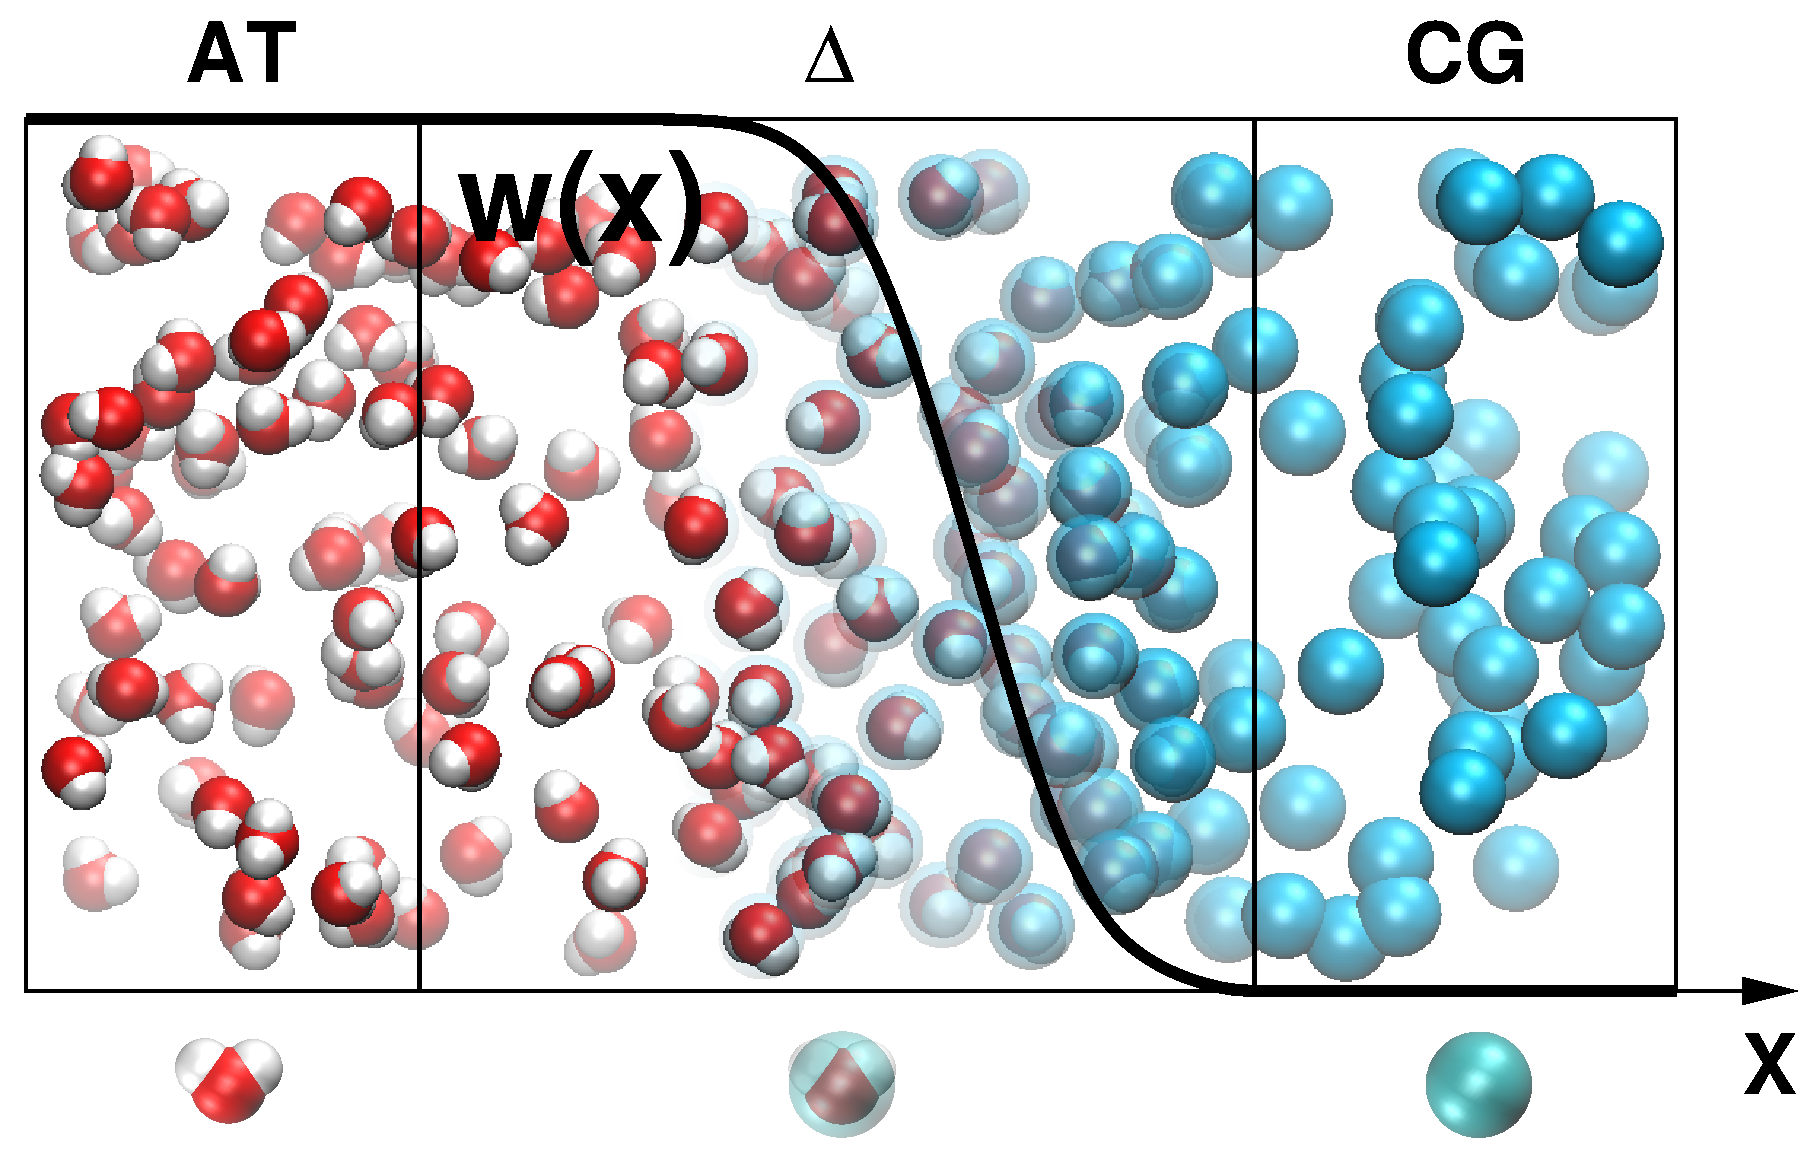
\includegraphics[width=0.8\textwidth]{fig/adapt-wat.eps}
  \end{figure}
  \vskip -.3cm
  \item<1-> Force interpolation scheme:
    \vskip -.6cm
  \begin{align*}
    {\vect F}_{\alpha \beta}&=w_\alpha w_\beta{\vect F}_{\alpha\beta}^{\AT}+[1-w_\alpha w_\beta]{\vect F}^{\CG}_{\alpha\beta} \bluec{\:+\: w_\alpha w_\beta (1-w_\alpha w_\beta)\vect F_{\alpha\beta}^{\rdf}}\\
    {\vect F}_{\alpha }& = \sum_{\beta}{\vect F}_{\alpha \beta} \bluec{\:+\:\vect F^\thf_{\alpha}}
  \end{align*}

  \end{itemize}
  % \footnote{M. Praprotnik, L. Delle Site, K. Kremer, JCP \textbf{123}, 224106 (2005)}
\end{frame}


\begin{frame}{AdResS: grand-canonical-like MD simulation}
  \begin{figure}
    \centering 
    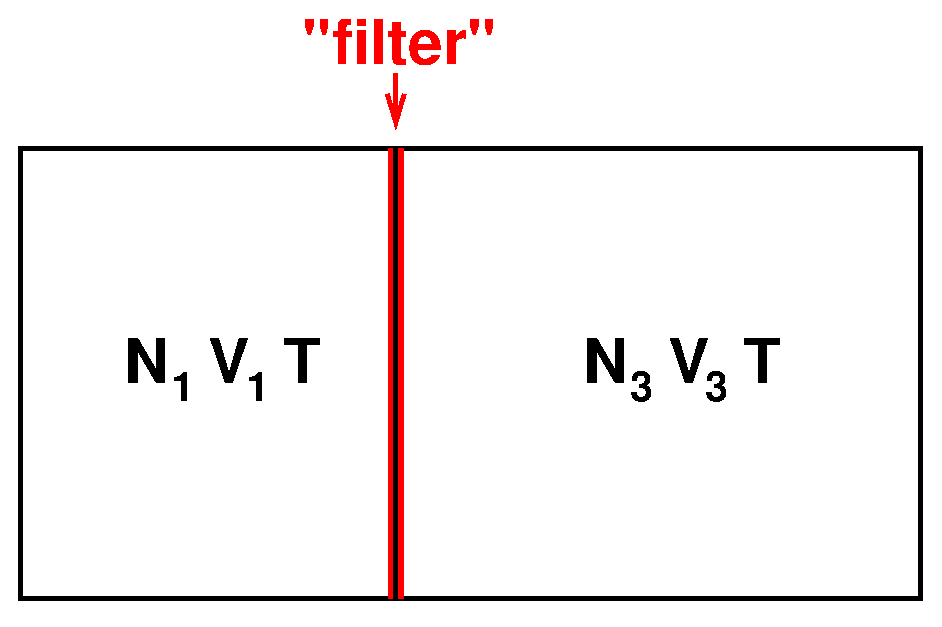
\includegraphics[width=0.5\textwidth]{fig/system/partition.eps}
    % 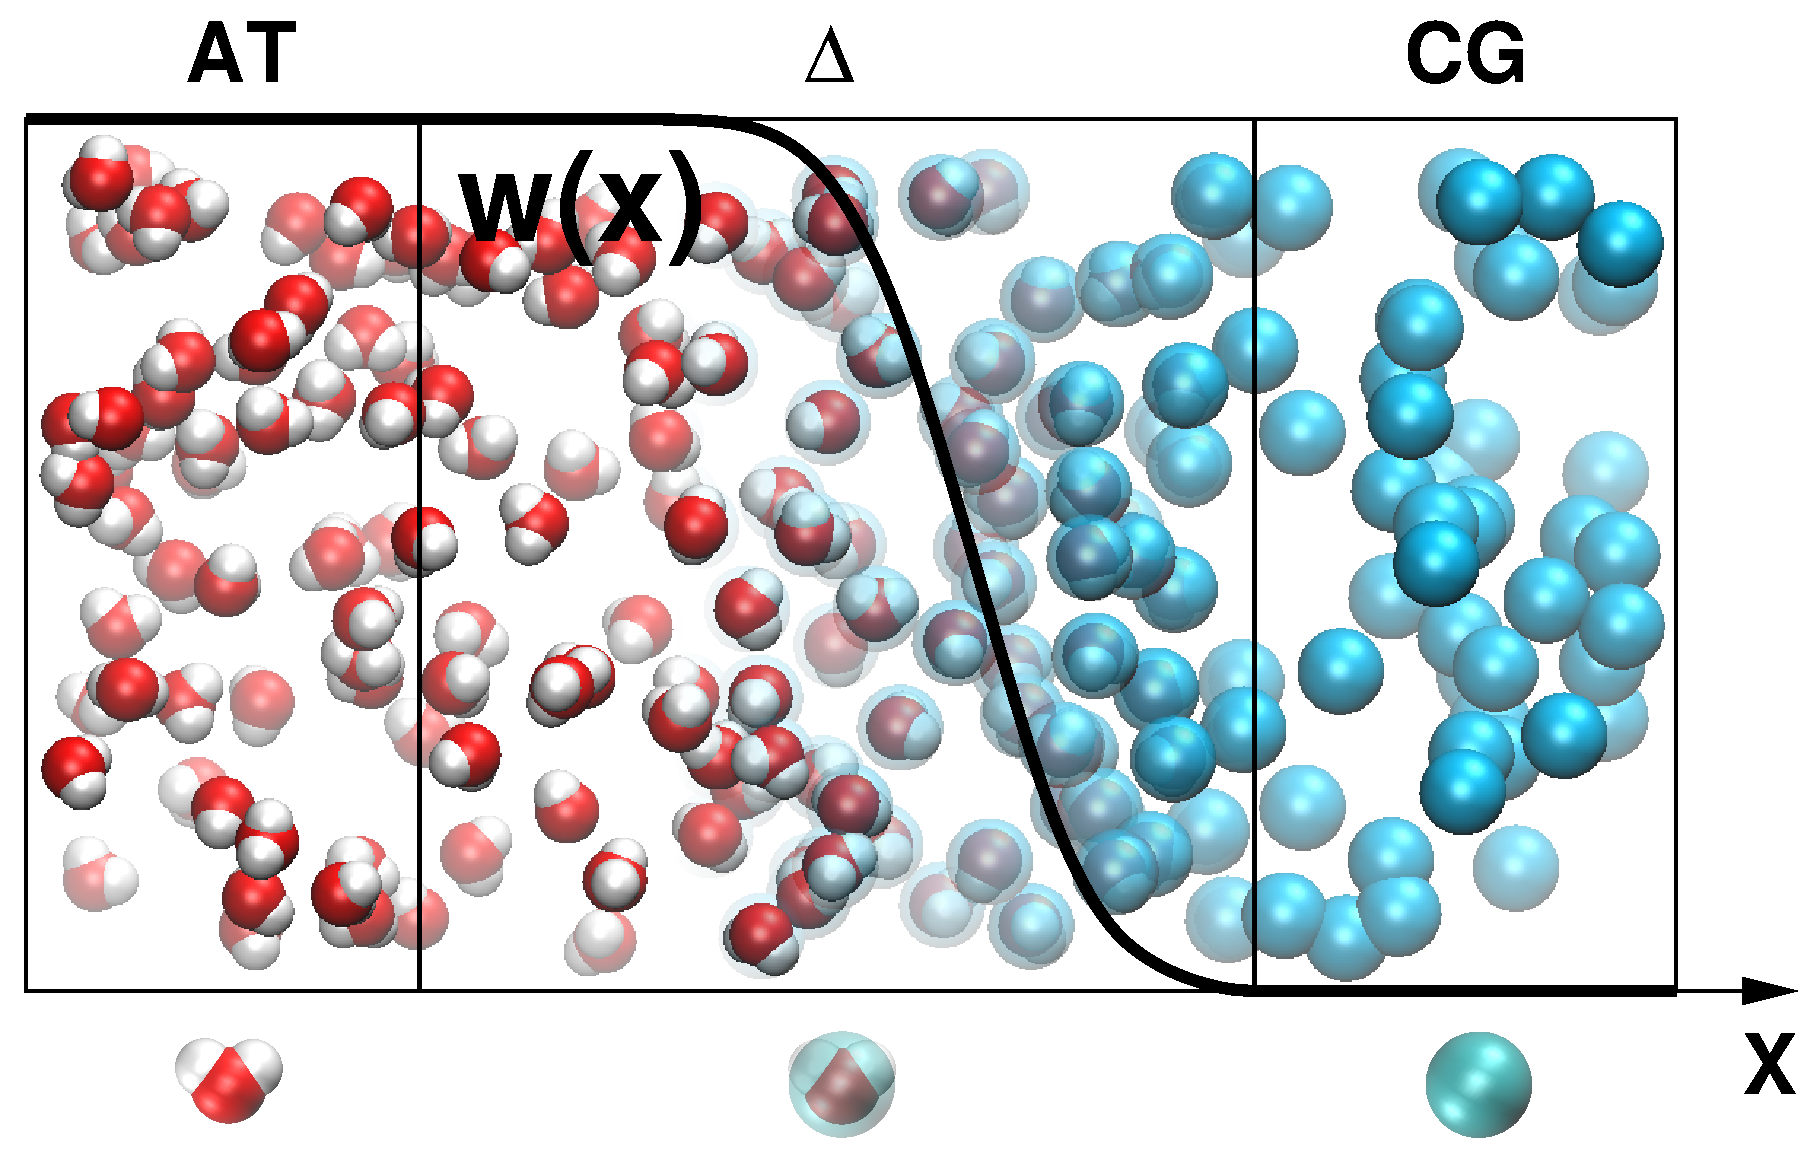
\includegraphics[width=0.8\textwidth]{fig/adapt-wat.eps}
  \end{figure}
  \begin{itemize}
  \item<1-> High-resolution region: system of interest.
  \item<2-> Low-resolution region: infinitly large particle reservior.
  \item<3-> Hybrid-resolution region: infinitly thin filter.
  \item<4-> Do we have the grand-canonical distribution?
    \bluec{
      \begin{align*}
        p(\vect x_\AT, N_\AT) = \frac{1}{\mathcal Z_\EX}
        e^{\beta\mu_{EX} N_\AT - \beta \mathcal H^{EX}(\vect x_\AT)} 
      \end{align*}}
  \item <5-> Decomposition:
    \bluec{
    \begin{align*}
      p(\vect x_\AT, N_\AT) = p(\vect x_\AT | N_\AT) \,{p (N_\AT)}
    \end{align*}}
  \end{itemize}
\end{frame}


\begin{frame}{AdResS: grand-canonical-like MD simulation}{Necessary conditions}
  \hfill
  \begin{minipage}[c]{0.60\linewidth}
    \begin{figure}
      \centering 
      \includegraphics[width=0.85\textwidth]{fig/system/at-equiv.eps}
      % 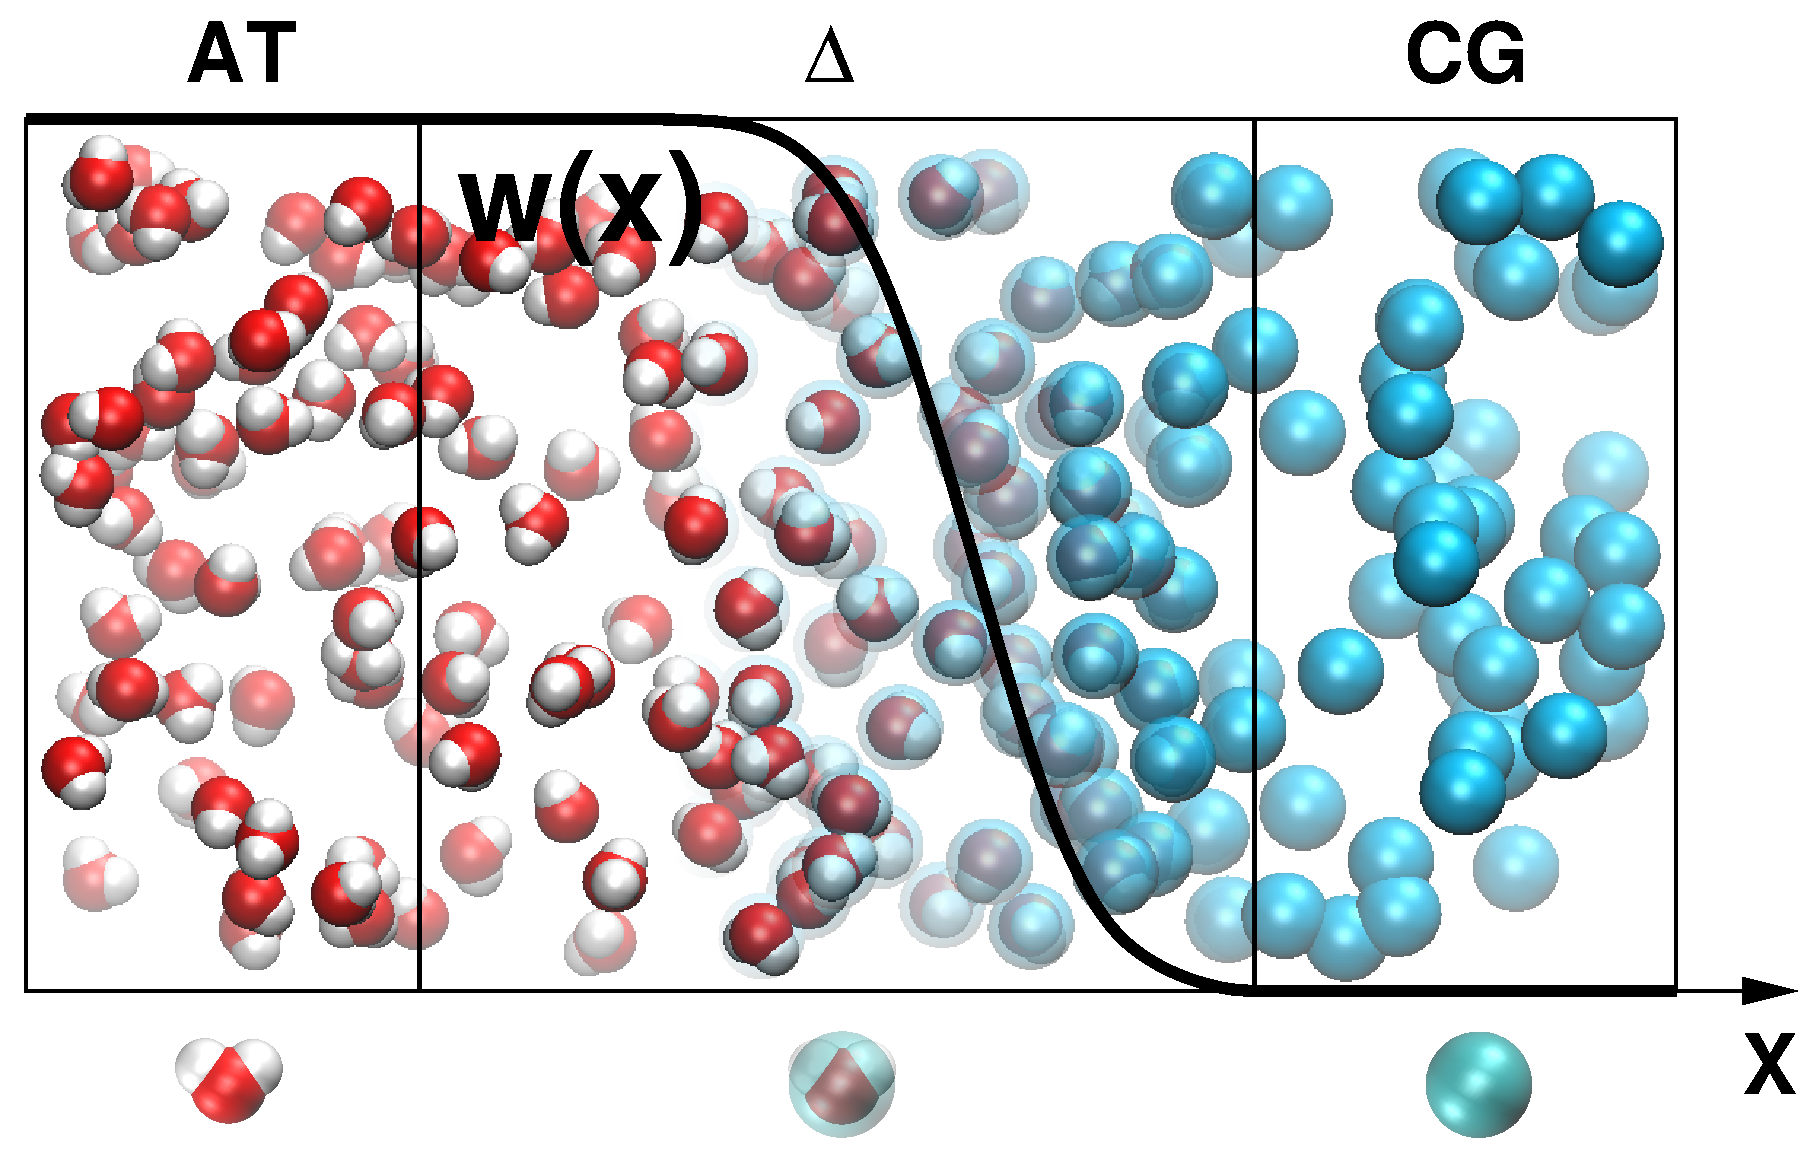
\includegraphics[width=0.8\textwidth]{fig/adapt-wat.eps}
    \end{figure}      
  \end{minipage}
  \hfill
  \begin{minipage}[c]{0.34\linewidth}
    \small{Accuracy of} \bluec{$p(\vect x_\AT | N_\AT) $}\\
    \vfill
    \whitec{
    Necessary conditions\\
    First order:\\
    {$\rho_{\HY} = \rho_\EX$}\\
    {\footnotesize{Thermodynamics force}}
    \vskip .2cm
    Second order:\\
    {$g_{\HY}(r) = g_\EX(r)$}\\
    {\footnotesize{RDF correction}}
    \vskip .2cm
    Third order:\\
    {$\corr_\HY = \corr_\AT$}\\
    {\footnotesize{Numerically verified}}
    }
  \end{minipage}
  \hfill
\end{frame}

\begin{frame}{AdResS: grand-canonical-like MD simulation}{Necessary conditions}
  \hfill
  \begin{minipage}[c]{0.60\linewidth}
    \begin{figure}
      \centering 
      \includegraphics[width=0.85\textwidth]{fig/system/at-equiv.eps}
      % 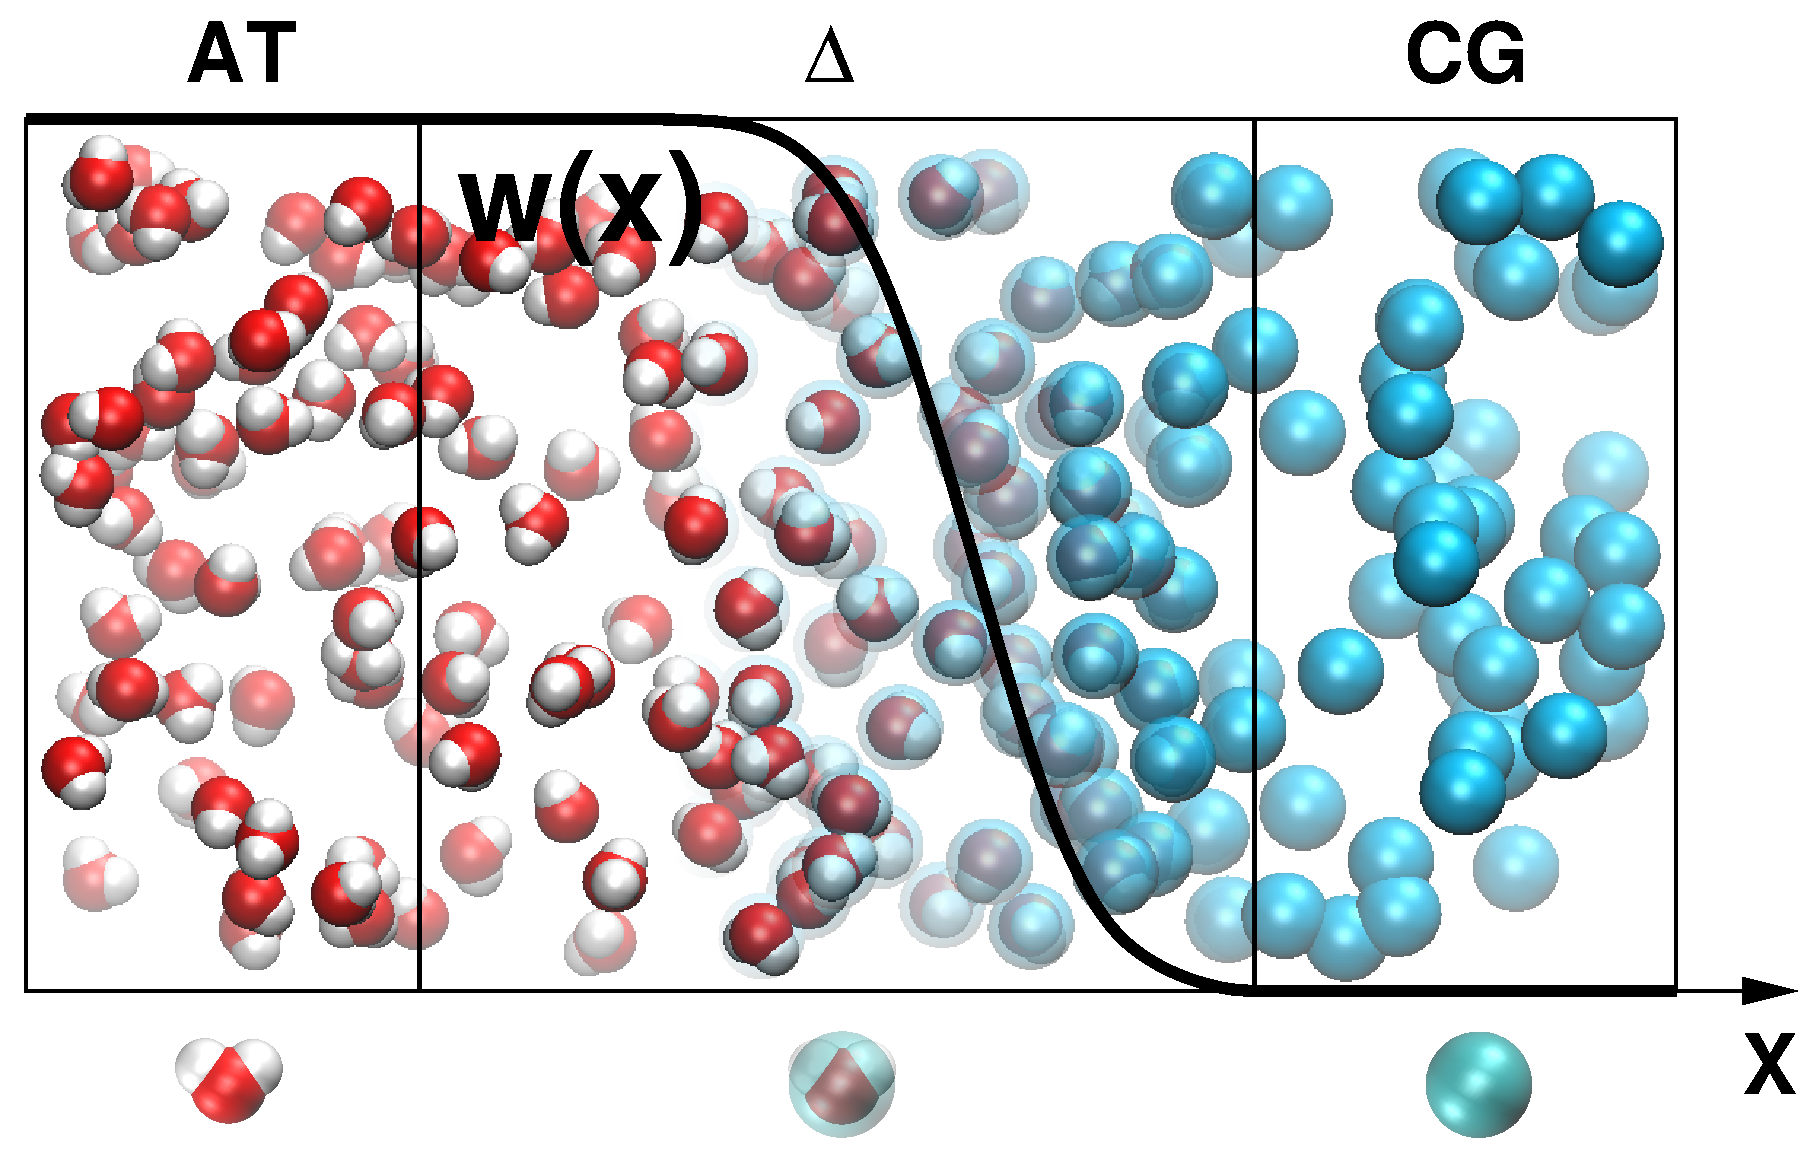
\includegraphics[width=0.8\textwidth]{fig/adapt-wat.eps}
    \end{figure}      
  \end{minipage}
  \hfill
  \begin{minipage}[c]{0.34\linewidth}
    \small{Accuracy of} \bluec{$p(\vect x_\AT | N_\AT) $}\\
    \vfill
    Necessary conditions\\
    First order:\\
    \bluec{$\rho_{\HY} = \rho_\EX$}\\
    \redc{\footnotesize{Thermodynamics force}}
    \vskip .2cm
    Second order:\\
    \bluec{$g_{\HY}(r) = g_\EX(r)$}\\
    \redc{\footnotesize{RDF correction}}
    \vskip .2cm
    Third order:\\
    \bluec{$\corr_\HY = \corr_\EX$}\\
    \redc{\footnotesize{Numerically verified}}
  \end{minipage}
  \hfill
\end{frame}

\begin{frame}{AdResS: grand-canonical-like MD simulation}{Necessary conditions}
  \begin{itemize}
    \vfill
  \item<1-> Accuracy of \bluec{$p(N_\AT) $}
    \vfill
  \item<2-> Necessary conditions
    \begin{itemize}
    \vfill
    \item<3-> First order: \redc{$ w_0 = \mu_{\CG} - \mu_{\AT}$}\\
      $w_0$: the work of the filter.
      \vfill
    \item <4-> \redc{$ w_0 = w_\thf + w_{\textrm{Q}}$}\\
      $w_\thf$ and $w_{\textrm{Q}}$ can be calculated by simulation.
    \vfill
    \item<5-> Second order: \redc{$\kappa_\AT = \kappa_{\CG}$}
    \end{itemize}
    \vfill
  \end{itemize}  
\end{frame}




\begin{frame}{WCA particles as a generic particle and energy reservior}
  \begin{itemize}
  \item<1-> Use WCA particles as CG molecules. 
  \item<2-> No need for coarse-graining.
  \item<3-> Even higher speed up.
  \item<4-> Theoretically fist order accuracy
  \item<5-> Numerically second order accuracy
  \item<6-> three-body correlation:
  \begin{figure}
    \centering 
    \includegraphics[width=0.9\textwidth]{fig/fig-wca-rdf3-diff-ex-hy1.eps}
  \end{figure}    
  \end{itemize}
\end{frame}

\begin{frame}{AdResS vs. insertion particle method (IPM)}
  \vfill
    \centering
    \begin{tabular}{l|l|c|l}
      & Sys. size ($\textsf{nm}^3$)
      & Traj. (\textsf{ns})
      & CPU time (hours)\\    \hline
      AdResS   &$29.9\times3.7\times3.7$ & 1 & 3.1\\
      IPM & $3.7\times3.7\times3.7$ & 8 & 4.5 (traj.) + 36.7 (IPM)\\
    \end{tabular}
  
  \vfill
  \begin{itemize}
  \item<1-> IPM: \redc{Single insertion} at each test.\\
    $10^5 \textrm{(position)} \times 10^5 \textrm{(orientation)}$ test insertions every 0.2ps.\\
    Still not converged.
    \vfill
  \item<1-> AdResS: \redc{Multiple insertions}.\\
    23 trials per ps. 832 out of 13824 molecules inserted in 1ns.\\
    Thermodynamic equilibrium reached.
    \vfill
  \item<2-> Excess chemical potential of water: (-23.5 kJ/mol)\\
    AdResS: -22.8 kJ/mol (3.0\%)\\
    IPM: \ \quad-24.6 kJ/mol (4.7\%) (400 ns traj. !)
  \end{itemize}
  % \caption{Comparison of computational efficiency.
  %     The AdResS simulation contains 13824 molecules, while the full atomistic (EX)
  %     water simulations contain 1728 molecules. In the AdResS simulation,
  %     the size of the AT + HY regions ($6.7\times3.7\times3.7\textsf{nm}^3$) is even larger than that of the EX water
  %     simulation box, so that we are actually in a {\it ``worst scenario''} situation. Moreover simulations with smaller reservoirs  gave essentially the same results reported for this system.
  %     ``Sys. size'' means the size of the box used in the simulation.
  %     ``Traj. length'' means the equilibrium trajectory
  %     used for the particle insertion in the IPM approach. Along the trajectories, frames
  %     of configurations were recorded every 0.2~\textsf{ps}.
  %     ``CPU time'' the is wall clock time spend on the simulation.
  %     For the particle insertion simulation, the CPU time is counted by two
  %     parts: the time of generating the equilibrium trajectories (traj.) (not expensive)
  %     and the time required by the IPM procedure (very expensive). Moreover, not only the insertion procedure is expensive on itself, but even after $8\textsf{ns}$ the insertion process has not actually converged. Simulations on longer time scales show that the full convergence is actually never reached, which suggests that the insertion procedure for a molecule as simple as water is not fully rigorous from the physical point of view.
  %   }
\end{frame}

\begin{frame}{Acknowledgement}
  \vfill
  The authors:
  \begin{itemize}
  \item Luigi Delle Site (FUB)
  \item Carsten Hartmann (FUB)
  \item Christof Sch\"utte (FUB)
  \end{itemize}
  \vfill
  For more details:
  \begin{itemize}
  \item H. Wang, C. Hartmann, C. Sch\"utte and L. Delle Site,\\
    \textbf{Phys. Rev. X}, 3, 011018, (2013).
  \item H. Wang, C. Sch\"utte and L. Delle Site,\\
    \textbf{J. Chem. Theory \& Compt.}, 8(8), 2878-2887 (2012).
  \end{itemize}
  \vfill
\end{frame}

\begin{frame}
  \vfill
  \begin{figure}
    \centering 
    \includegraphics[width=0.88\textwidth]{fig/system.cover/main.eps}
  \end{figure}
  \vskip -.5cm
  \footnotesize{
    1, Phys. Rev. X, 3, 011018, (2013).\\
  \vskip -.1cm
    2, J. Chem. Theory \& Compt., 8(8), 2878-2887 (2012).
  }
\end{frame}


\begin{frame}{Numerical verification}{Density profile}
  \begin{figure}
    \centering 
    \includegraphics[width=0.8\textwidth]{fig/fig-rho.eps}
  \end{figure}  
\end{frame}

\begin{frame}{Numerical verification}{Fluctuation}
  \begin{figure}
    \centering 
    \includegraphics[width=0.8\textwidth]{fig/fig-count.eps}
  \end{figure}  
\end{frame}

\begin{frame}{Numerical verification}{RDFs}
  \begin{figure}
    \centering 
    \includegraphics[width=0.6\textwidth]{fig/fig-rdf-all-375-425.eps}
  \end{figure}  
\end{frame}

\begin{frame}{Numerical verification}{RDFs}
  \begin{figure}
    \centering 
    \includegraphics[width=0.6\textwidth]{fig/fig-rdf-all-425-516.eps}
  \end{figure}  
\end{frame}

\begin{frame}{Numerical verification}{RDFs}
  \begin{figure}
    \centering 
    \includegraphics[width=0.6\textwidth]{fig/fig-rdf-all-516-608.eps}
  \end{figure}  
\end{frame}

\begin{frame}{Numerical verification}{RDFs}
  \begin{figure}
    \centering 
    \includegraphics[width=0.6\textwidth]{fig/fig-rdf-all-608-700.eps}
  \end{figure}  
\end{frame}


\begin{frame}{Numerical verification}{Three-body correlation}
  \begin{figure}
    \centering 
    \includegraphics[width=0.9\textwidth]{fig/fig-rdf3-diff.eps}
  \end{figure}  
  Definition
  \tiny{\bluec{
    \begin{align*}
      \corr (\vect s_1, \vect s_2, \vect s_3)
      =
      \frac1{\rho(\vect s_1)\rho(\vect s_2)\rho(\vect s_3)}
      \big\langle
      (\hat\rho(\vect s_1) - \rho(\vect s_1))\cdot
      (\hat\rho(\vect s_2) - \rho(\vect s_2))\cdot
      (\hat\rho(\vect s_3) - \rho(\vect s_3))
      \big\rangle
    \end{align*}}}
\end{frame}

\begin{frame}{Convergence of the IPM}
  \begin{figure}
    \centering 
    \includegraphics[width=0.8\textwidth]{fig/fig-tpi.eps}
  \end{figure}  
\end{frame}



\end{document}
